% C5. Qué revela el modelo sobre los precios (interpretación hedónica)
\begin{frame}{Qué revela el modelo: el precio es tamaño, ubicación y lo que dice el anuncio}
  \centering
  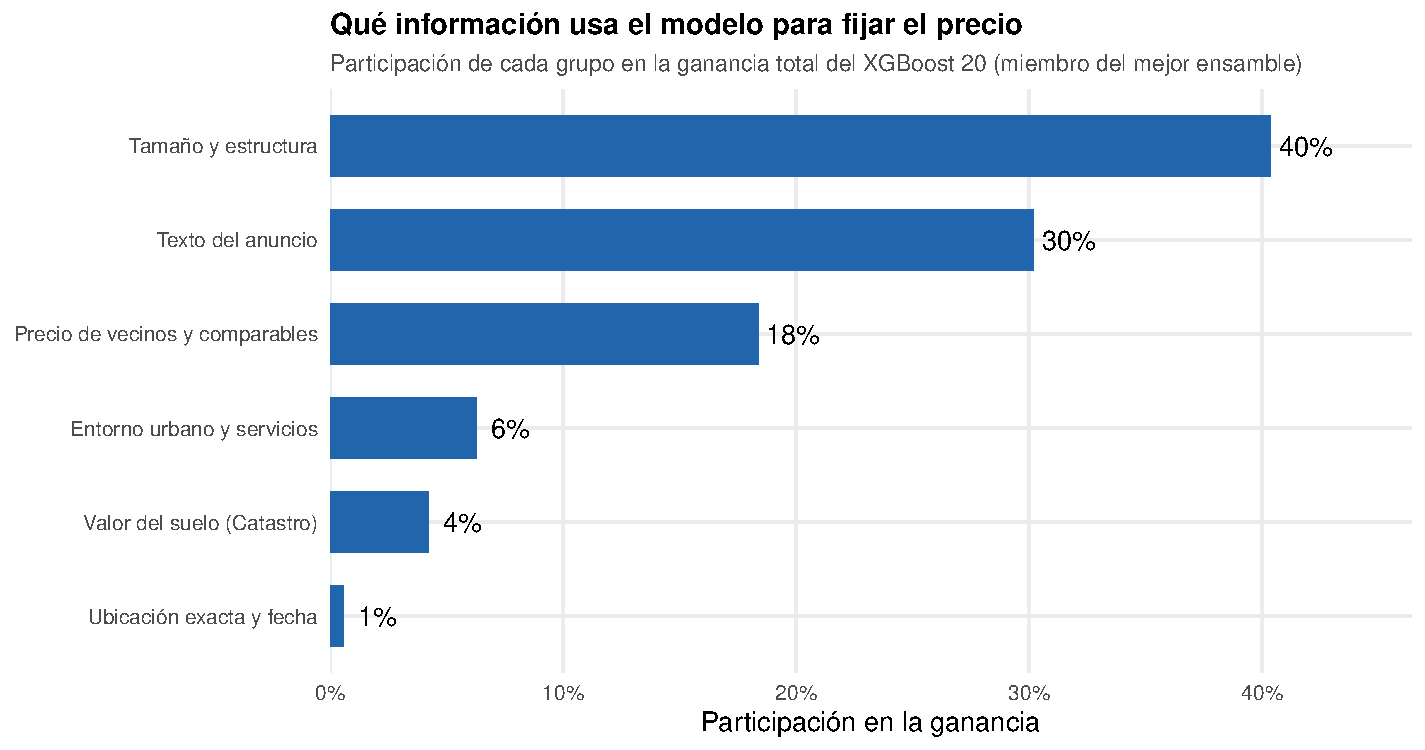
\includegraphics[height=0.8\textheight]{pres_importancia_grupos.pdf}
  \lectura{Como en Rosen (1974), el precio depende de las características de la vivienda y de su entorno. El texto recoge calidad y acabados que ninguna otra variable mide.}
  \note{La ganancia mide cuánto mejora el ajuste cada vez que el modelo usa una variable. El tamaño (área, baños, habitaciones) explica el nivel del precio. El texto es el segundo grupo: dice si el inmueble es de lujo, está remodelado o tiene club house. El precio de los vecinos y el valor del suelo de Catastro resumen la ubicación. Las amenidades sueltas (parques, transporte) pesan poco por separado, porque su efecto ya está en el precio de la zona.}
\end{frame}
